\chapter{Разработка программных модулей системы электронного обучения и результаты экспериментов} \label{chapt4}

\section{Архитектура системы электронного обучения на основе онтологий} \label{sect4_1}

Для реализации описанных алгоритмов, методов и методик была разработана система электронного обучения ECOLE (Enhanced Course Ontology for Linked Education). Кроме основных функций системы электронного обучения ECOLE выполняет функции семантического агрегатора открытых образовательных ресурсов.

Основными функциями системы ECOLE являются:

\begin{itemize}
\item сбор учебных материалов из внешних источников и преобразование их в структурированный формат;
\item предоставление данных пользователям в различных форматах (текст, графика, мультимедиа);
\item предоставление данных сторонним приложениям по работе с Linked Data (SPARQL-endpoint);
\item возможность редактирования и создания новых учебных материалов и изменение образовательных процессов;
\item связывание учебных материалов со сторонними источниками (электронные библиотеки, мультимедиа ресурсы, социальные сети);
\item анализ актуальности учебных материалов и курсов (обновление данных полученных из внешних источников);
\item анализ полноты и сбалансированности учебных материалов (покрытия модуля тестами, рейтинговая система оценки материалов);
\item поиск учебных материалов;
\item разграничение доступа к редактированию информации различным группам пользователей.
\end{itemize}

Сервер системы электронного обучения ECOLE основан на платформе Information Workbench. Платформа Information Workbench предоставляет функционал для работы с открытыми связными данными Linked Open Data. Платформа основана на использовании программных модулей с открытым исходным кодом. Пользовательский интерфейс сервера ECOLE основан на модуле семантической разметки Semantic MediaWiki. Данный модуль позволяет использовать переопределенные шаблоны и визуальные средства для отображения семантических данных в виде Wiki-страниц. Редактирование и управление RDF данными системы реализовано с использованием платформы OpenRDF Sesame. Сервер системы ECOLE поддерживает запросы SPARQL. Сервер предоставляет открытую точку доступа для SPARQL запросов.

Внешним интерфейсом системы электронного обучения ECOLE является облегченная система управления образованием Learning Management System (LMS). LMS предназначена для удобного представления учебных материалов пользователям системы. LMS обладает локальным хранилищем и производит управление пользовательскими данными, настройками и результатами обучения студентов. Внешний интерфейс системы предоставляет функционал по администрированию системы и управлению доступом к данным системы. В LMS реализованы модули для отображения видео-лекций, слайдов, тестов и практических заданий.

Внешний интерфейс взаимодействует с сервером системы с помощью запросов к открытой точке доступа SPARQL. Внешний интерфейс получает с сервера данные по учебным материалам и отношениям между объектами курса. Приватные персональные данные пользователей и настройки LMS хранятся в локальной памяти внешнего интерфейса.

Общая архитектура системы электронного обучения ECOLE представлена на рисунке \ref{img:overall_arch}.

\begin{figure} [h] 
  \center
  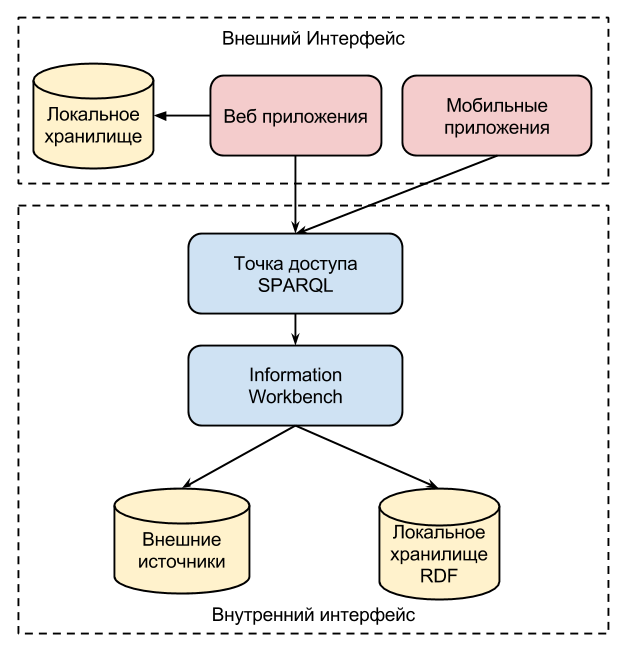
\includegraphics [scale=0.6] {overall_arch}
\caption{Общая архитектура системы электронного обучения ECOLE.}
  \label{img:overall_arch}  
\end{figure}

LMS реализована на языке Python с использованием Django Web Framework  \cite{holovaty2009definitive}. Библиотека SPARQLWrapper использована отправки запросов к точке доступа SPARQL. Когда пользователь завершает тест, LMS собирает результаты теста, ответы на задания и дополнительную статистику и записывает полученные данные на сервер с помощью запроса SPARQL Update Query \cite{seaborne2008sparql}. В результате прохождения теста студентом на сервере создается объект класса <<AttemptToPassTest>> (Попытка) с набором правильных и неправильных ответов на задания теста. Данный объект связывается с объектом студента. В целях безопасности персональных данных объекты студентов идентифицируются с использованием хеш-суммы электронной почты студента.

После прохождения теста система предоставляет студенту информацию о количестве и доле правильных ответов на задания теста. Так же студенту предоставляется список концептов предметной области для повторения. Система генерирует список проблемных концептов для студента, используя результаты теста и связи между концептами системы и заданиями теста. Для каждого концепта предметной области, связанного с заданиями теста, производится расчет рейтинга на основе ответов студента. Лист проблемных концептов сортируется в порядке возрастания рейтинга. Чем выше рейтинг концепта, тем больше правильных ответов дал студент на задания связанные с данным концептом и тем меньше затруднений вызвал у студента данный концепт. Рейтинг концепта, полученный в контексте прохождения теста, может быть отражен в глобальном рейтинге знаний концептов студентом. Глобальный рейтинг знаний для каждого концепта позволяет студенту выявлять проблемные концепты и восполнять знания по ним.   


\section{Описание пользовательских интерфейсов разработанной системы электронного обучения} \label{sect4_2}

%%%%%%%

%% СКРИНШОТЫ И ОПИСАНИЕ СИСТЕМЫ

%%%%%%%

\section{Метод преобразования онтологий системы электронного обучения в формат SCORM} \label{sect4_3}

Учебные материалы хранящиеся в семантическом формате не могут быть интегрированы системы электронного обучения без поддержки семантических технологий. Данный факт не позволяет системе ECOLE экспортировать агрегированные учебные материалы в окружение сисем электронного обучения университетов. В данный момент существуют стандарты позволяющие интегрировать и обмениваться учебными материалами между системами электронного обучения. Одним из таких стандартов является стандарт SCORM. Для реализации конвертации и экспорта учебных материалов из семантического формата в формат SCORM был разработан программный модуль преобразования. Экспортирование данных из системы ECOLE в формат SCORM позволит интегрировать учебные материалы в большое количество типов систем электронного обучения, поддерживающих стандарт SCORM. Одной из таких систем является популярная ситсема электронного обучения Moodle.

Разработанный модуль решает следующий ряд задач:

\begin{itemize}
\item извлечение данных в семантических форматах из ситсемы электронного обучения на основе семантических технологий;
\item создание учебных материалов из извлеченных данных по предопределенным шаблонам;
\item генерация данных из учебных материалов в соответствии со стандартом SCORM;
\item поддержка различных интерфейсов управления модулем, таких как  пользовательский интерфейс или REST API.
\end{itemize}

Разработанный модуль использует сервисы и программные модели платформы Information Workbench. В основе модуля лежит Сервис Преобразования SCORM. Данный сервис взаимодействует с различными модулями сервера и интерфейс системы ECOLE для извлечения учебных материалов и их преобразования в формат SCORM. Модуль реализован на языке Java и интегрирован в платформу Information Workbench. Архитиктура программного модуля представлена на рисунке \ref{img:overall_scorm_arch}.

\begin{figure} [h] 
  \center
  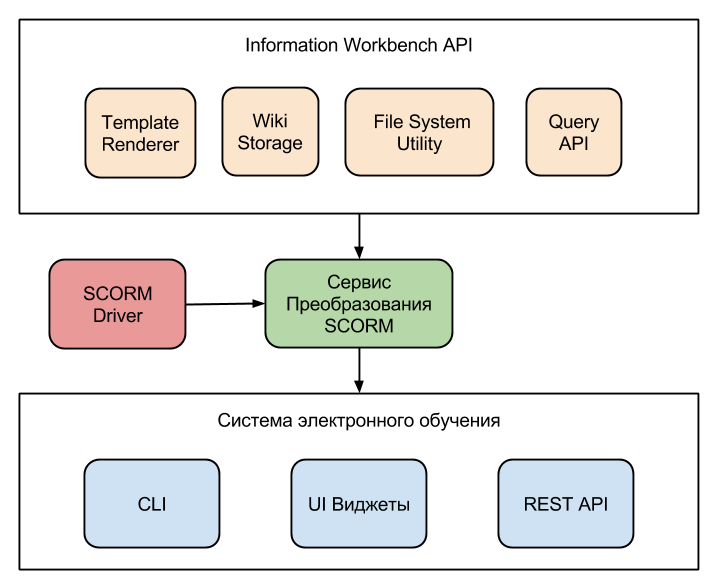
\includegraphics [scale=0.65] {overall_scorm_arch}
\caption{Архитектура программного модуля преобраования данных в формат SCORM в системе ECOLE.}
  \label{img:overall_scorm_arch}  
\end{figure} 

Сервис Преобразования SCORM использует модуль Query API для сбора семантических данных. Для сбора предопределенных шаблонов используется сервис Wiki Storage. Программный модуль Template Renderer используется для генерации HTML страниц из собранных учебных материалов по преопределенным шаблонам. File System Utility используется для управления файлами и директориями системы. Для генерации данных в формате SCORM используется внешняя библиотека SCORM Driver. В качестве интерфейса Сервиса Преобразования SCORM могут выступать пользовательские <<виджеты>>, REST API и интерфейс командной строки (CLI).


Метод преобразования учебных материалов в формат SCORM заключается в формировании набора HTML страниц на основе шаблонов и семантических данных. Для создания SCORM пакета необходимы следующие шаблоны:

\begin{itemize}
\item шаблон начальной страницы электронного курса;
\item шаблон лекции;
\item шаблон заключительной страницы электронного курса.
\end{itemize}

При генерации каждный шаблон получает информацию о соответсвующем объекте онтологии. Шаблоны начальной и заключительной страницы курса получают информацию об объекте электронного курса. Шаблон лекции получает информацию об объекте лекции электронного курса. В результате генерации формируются HTML страницы с данными переданных объектов. Алгоритм преобразования семантически данных учебных материалов в формат SCORM представлен на рисунке \ref{img:overall_scorm_algo}.

\begin{figure} [h] 
  \center
  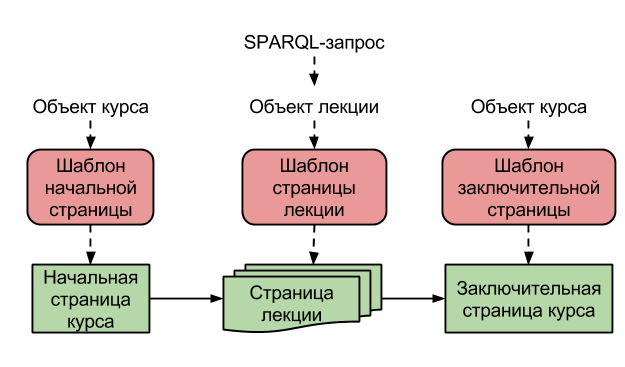
\includegraphics [scale=0.7] {overall_scorm_algo}
\caption{Алгоритм преобразования семантически данных учебных материалов в формат SCORM.}
  \label{img:overall_scorm_algo}  
\end{figure} 

Данные об объектах собираются с помощью запросов SPARQL. Шаблоны описываются с помощью синтаксиса Semantic MediaWiki. Шаблоны поддерживают разметку HTML. В ходе генерации учебных материалов в формате SCORM Сервисом Преобразования SCORM  производиться дополнительное наполнение заголовков HTML страниц и извлечение медиа ресурсов из содержания учебных материалов. Ниже представлен пример описания шаблона  лекции для разработанного программного модуля. 

\begin{lstlisting}
= $this.rdfs:label$ =

=== About ===

'''Module''': $this.learningRu:isLectureOf$
'''Number of lecture''': $this.learningRu:numberOfLecture$ 

=== Terms ===

{{#sparql: SELECT DISTINCT ?label
 WHERE { ?term learningRu:isTermOf {{this}} . 
 ?term rdfs:label ?label } } 
 | format=template  | template=Template:ListTemplate}}

\end{lstlisting}

Разработанный программный модуль позволяет преподавателям и авторам экспортировать из системы ECOLE электронные курсы в формат SCORM для дальнейшей интеграции в другие системы электронного обучения. 

\section{Результаты применения методики агрегации данных в системе электронного обучения} \label{sect4_4}

Основной набор данных системы дистанционного обучения ECOLE формировался вручную. Часть данных была создана с помощью методов наполнения онтологии описанных в главе 3. Набор данных системы состоит из объектов образовательного процесса, таких как курс, модуль, лекция, тест, практика, предметный термин, предметная область и книга. В результате работы NLP  алгоритмов по извлечению предметных терминов из тестов были получены результаты, представленные в таблице \ref{table:nlp_resutls}. С одной стороны с терминами было связано 95\% заданий тестов. С другой стороны более 50\% терминов курса остались не связанными с заданиями тестов. Одной из причин данного явления является косвенное употребление предметных терминов в задании. Чтобы решить такое задание необходимо знать предметный термин, который не упомянут ни в тексте задания, ни в тексте ответов. Примером таких заданий являются задачи на поиск длинны гипотенузы треугольника при известных катетах. Косвенно связанным предметным терминов в данном примере является термин «Теорема Пифагора». В текущей реализации метода извлечение косвенных терминов не производится. В будущем планируется использование семантических связей между терминами для выявления косвенных предметных терминов в заданиях тестов.

\begin{table}[h!]
\centering
\caption{Результаты работы алгоритмов обработки естественного языка по извлечению предметных терминов из тестов.)}
\label{table:nlp_resutls}
\begin{tabular}{ |p{12cm}|c|  }
\hline Количество обработанных заданий & 20 \\
\hline Процент связанных заданий, \% & 95 \\
\hline Процент несвязанных заданий, \% & 5 \\
\hline Количество извлеченных терминов-кандидатов & 155 \\
\hline Количество терминов извлеченных вручную & 30 \\
\hline Термины системы, совпавшие с терминами-кандидатами, \% & 50 \\
\hline Термины-кандидаты, совпавшие с терминами системы, \% & 8 \\
\hline Термины-кандидаты, добавленные в систему после прохождения проверки, \%  & 6 \\
\hline Ложные термины-кандидаты, \% & 86 \\
\hline
\end{tabular}
\end{table}  


\section{Результаты применения методов анализа на учебных курса и группах студентов} \label{sect4_5}

Модуль автоматического расчета оценки и рейтинга знаний студента по предметным терминам и областям был разработан на языке Python и интегрирован в систему электронного обучения ECOLE с использованием Django Web Framework. Работа модуля была применена при прохождении студентами курса <<Интеллектуальные системы>>. В результате работы модуля было рассчитано значение для предметных терминов из области <<Экспертные системы>>. В данный момент в предметной области содержится 43 термина. Десять терминов с наибольшим значением представлены в таблице \ref{table:term_importance_result}. Полученные результаты демонстрируют значение предметных терминов в образовательном процессе. Для изучения предметных терминов одной области могут потребоваться знания терминов другой предметной области. Таким образом, значения терминов не зависят от предметных областей, к которым данные термины относятся. Расчеты показывают, что базовые понятия в предметной области не являются самыми важными в ней.    

\begin{table}
\centering
\caption{Значения предметных терминов области <<Экспертные системы>>}
\label{table:term_importance_result}
\begin{tabular}{|p{7cm}|c|}
\hline Предметный термин & Значение \\
\hline Инженерия знаний & 3.749703 \\
\hline Знания & 1.796706 \\
\hline Извлечение знаний & 1.796706 \\
\hline Рабочая память & 1.706427 \\
\hline Представление (репрезентация) знаний & 1.606853 \\
\hline Процесс разрешения конфликтов & 1.374309 \\
\hline Язык представления знаний & 1.191552 \\
\hline Экстенсионал & 1.169817 \\
\hline Интенсионал & 1.169817 \\
\hline Интуитивные знания & 1.169817 \\
\hline
\end{tabular}
\end{table}

При прохождении студентом  лекций и тестов модуль рассчитывает рейтинги предметных терминов и областей в соответствии с разработанными методами. В результате студенту демонстрируется список предметных областей и терминов с оценками. Интерфейс списка оценок представлен на рисунке \ref{fig:user_screen_result}.

\begin{figure} [h] 
  \center
  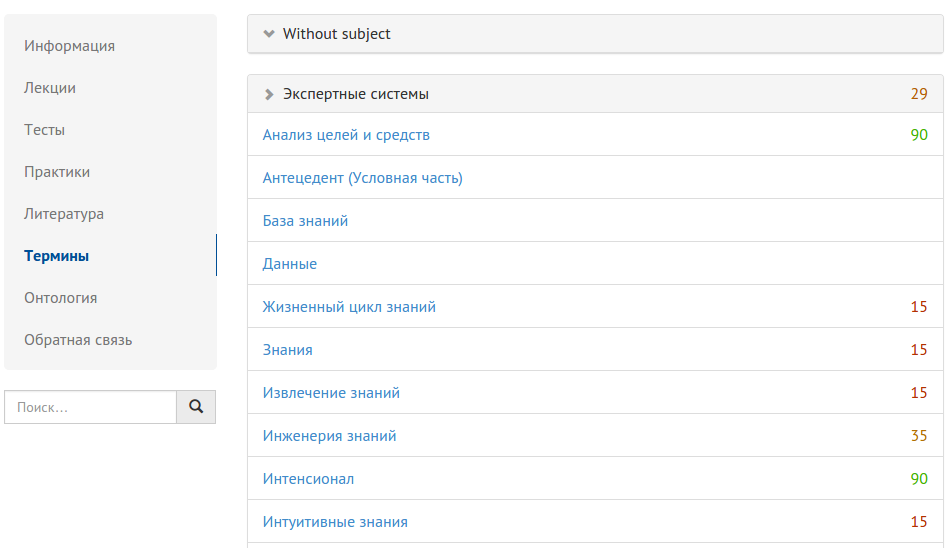
\includegraphics [scale=0.45] {user_screen_result}
  \caption {Интерфейс списка предметных областей и терминов с рейтингами знаний в системе ECOLE} 
  \label{fig:user_screen_result}
\end{figure}


%%%%%%%%

% НУЖНЫ РЕЗУЛЬТАТЫ ПО ОПРОСАМ СТУДЕНТОВ

%%%%%%%%

\clearpage